\documentclass[11pt]{article}
\usepackage{geometry}                
\geometry{letterpaper}                   





\usepackage[english]{babel}
\usepackage[utf8x]{inputenc}
\usepackage{amsmath}
\usepackage{tikz}
\usetikzlibrary{positioning}

\usetikzlibrary{arrows,automata}


%\usepackage[latin1]{inputenc}
\usepackage{graphicx}
\usepackage{amssymb}
\usepackage{epstopdf}
\usepackage{natbib}
\usepackage{amssymb, amsmath}
\DeclareGraphicsRule{.tif}{png}{.png}{`convert #1 `dirname #1`/`basename #1 .tif`.png}

\title{Airplane Boarding}
\author{Anton Schäfer, Nils Blach}
%\date{date} 

\begin{document}



\thispagestyle{empty}

\begin{center}

\includegraphics[width=5cm]{ETHlogo.eps}

\bigskip


\bigskip


\bigskip


\LARGE{ 	Lecture with Computer Exercises:\\ }
\LARGE{ Modelling and Simulating Social Systems\\}

\bigskip

\bigskip

\small{Project Report}\\

\bigskip

\bigskip

\bigskip

\bigskip


\begin{tabular}{|c|}
\hline
\\
\textbf{\LARGE{Insert Title Here}}\\
\textbf{\LARGE{...}}\\
\\
\hline
\end{tabular}
\bigskip

\bigskip

\bigskip

\LARGE{Name 1, Name 2  \& [...]}



\bigskip

\bigskip

\bigskip

\bigskip

\bigskip

\bigskip

\bigskip

\bigskip

Zurich\\
Dec 2018\\

\end{center}



\newpage

%%%%%%%%%%%%%%%%%%%%%%%%%%%%%%%%%%%%%%%%%%%%%%%%%

\newpage
\section*{Agreement for free-download}
\bigskip


\bigskip


\large We hereby agree to make our source code for this project freely available for download from the web pages of COSS. Furthermore, we assure that all source code is written by ourselves and is not violating any copyright restrictions.

\begin{center}

\bigskip


\bigskip


\begin{tabular}{@{}p{3.3cm}@{}p{6cm}@{}@{}p{6cm}@{}}
\begin{minipage}{3cm}

\end{minipage}
&
\begin{minipage}{6cm}
	\vspace{2mm} \large Anton Sch{\"a}fer

 \vspace{\baselineskip}

\end{minipage}
&
\begin{minipage}{6cm}

\large Nils Blach

\end{minipage}
\end{tabular}


\end{center}
\newpage

%%%%%%%%%%%%%%%%%%%%%%%%%%%%%%%%%%%%%%%



% IMPORTANT
% you MUST include the ETH declaration of originality here; it is available for download on the course website or at http://www.ethz.ch/faculty/exams/plagiarism/index_EN; it can be printed as pdf and should be filled out in handwriting


%%%%%%%%%% Table of content %%%%%%%%%%%%%%%%%

\tableofcontents

\newpage

%%%%%%%%%%%%%%%%%%%%%%%%%%%%%%%%%%%%%%%



\section{Abstract}

\section{Individual contributions}
\paragraph{Model:} Both
\paragraph{Data Collection/Calculation:} Anton Sch{\"a}fer
\paragraph{Data Display/Graphs:} Nils Blach

\section{Introduction and Motivations}

\section{Description of the Model}

\begin{figure}
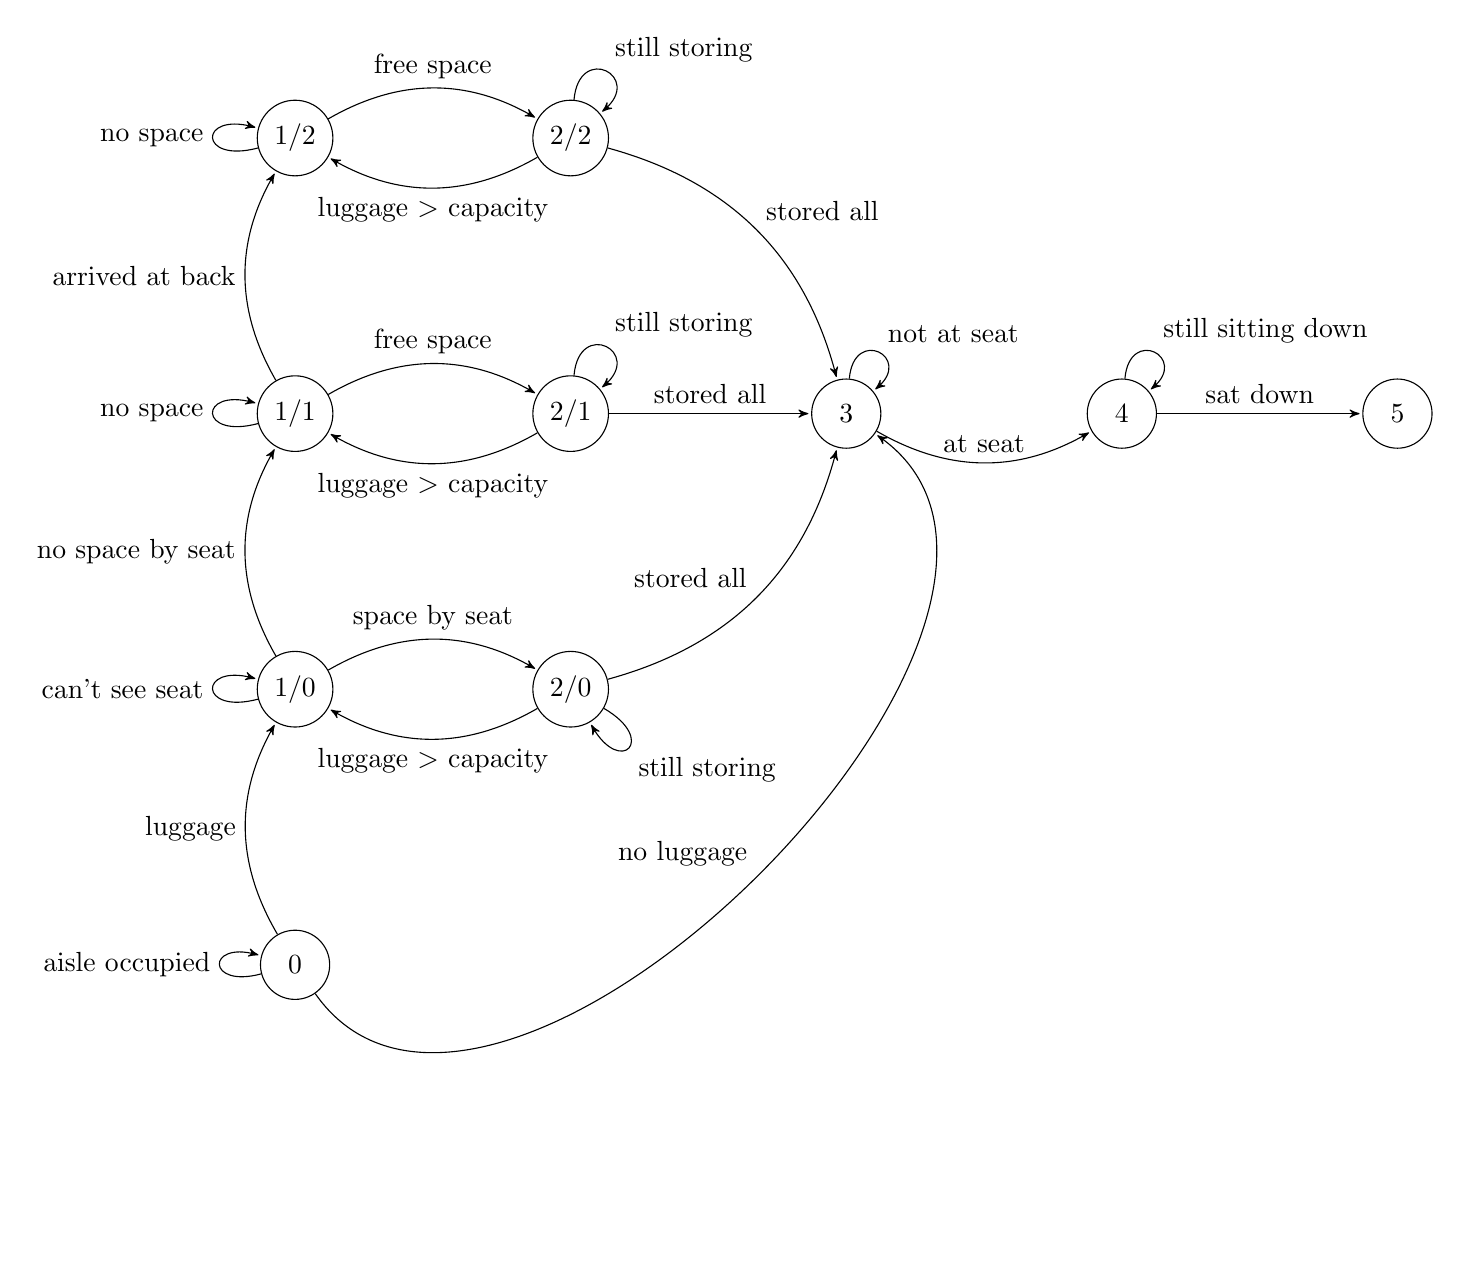
\begin{tikzpicture}[->,>=stealth',shorten >=1pt,auto,node distance=3.5cm,
        scale = 1,transform shape]

  \node[state] (0) [] {$0$};
  \node[state] (1/0) [above of=0] {$1/0$};
  \node[state] (1/1) [above of=1/0] {$1/1$};
  \node[state] (1/2) [above of=1/1] {$1/2$};
  \node[state] (2/0) [right of=1/0] {$2/0$};
  \node[state] (2/1) [right of=1/1] {$2/1$};
  \node[state] (2/2) [right of=1/2] {$2/2$};
  \node[state] (3) [right of=2/1] {$3$};
  \node[state] (4) [right of=3] {$4$};
  \node[state] (5) [right of=4] {$5$};

  \path (0) edge   [bend left]           node {luggage} (1/0)
        (0) edge  [bend right=100]            node {no luggage} (3)
        (0) edge  [loop left]            node {aisle occupied} (0)
        (1/0) edge  [loop left]            node {can't see seat} (1/0)
        (1/0) edge    [bend left]          node {no space by seat} (1/1)
        (1/0) edge   [bend left]           node {space by seat} (2/0)
        (1/1) edge  [loop left]            node {no space} (1/1)
        (1/1) edge   [bend left]           node {arrived at back} (1/2)
        (1/1) edge   [bend left]            node {free space} (2/1)
        (1/2) edge   [loop left]           node {no space} (1/2)
        (1/2) edge    [bend left]           node {free space} (2/2)
        (2/0) edge     [out=330,in=300,looseness=8]        node {still storing} (2/0)
        (2/0) edge    [bend left]          node {luggage $>$ capacity} (1/0)
        (2/0) edge     [bend right]         node {stored all} (3)
        (2/1) edge      [out=85,in=40,looseness=5]        node {still storing} (2/1)
        (2/1) edge     [bend left]         node {luggage $>$ capacity} (1/1)
        (2/1) edge              node {stored all} (3)
        (2/2) edge     [out=85,in=40,looseness=5]         node {still storing} (2/2)
        (2/2) edge     [bend left]         node {luggage $>$ capacity} (1/2)
        (2/2) edge     [bend left]         node {stored all} (3)
        (3) edge     [out=85,in=40,looseness=5]       node {not at seat} (3)
        (3) edge     [bend right]         node {at seat} (4)
        (4) edge      [out=85,in=40,looseness=5]         node {still sitting down} (4)
        (4) edge              node {sat down} (5);

\end{tikzpicture}
\end{figure}
 


\section{Implementation}

\section{Simulation Results and Discussion}

\section{Summary and Outlook}

\section{References}






\end{document}  



 
